\chapter{Basic Operational Amplifier Circuits}

Operational amplifiers are extremely useful and versatile circuits.
This chapter presents basic application circuits which use operational amplifiers for amplification, buffering, summing, integrating, etc.

The circuit schematics in this chapter also show a series input capacitor to block DC.
The capacitor and resistors should be chosen appropriately to block only the desired range of low frequencies, or the capacitor should be removed to process DC signals.

\section{Comparator}
\begin{center}
	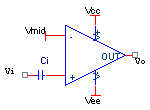
\includegraphics{schematics/comparator.PNG}
\end{center}
A comparator is a very simple circuit that compares its input voltage $v_{i}$ to a DC reference voltage $V_{REF}$ and outputs $V_{CC}$ if $v_{i} > V_{REF}$ and $V_{EE}$ otherwise. It utilizes the operational amplifier's ideally infinite open loop gain to to force $v_{o}$ to $V_{CC}$ or $V_{EE}$ for even a very small input differential voltage ($v_{i} - V_{REF}$).

\section{Inverting amplifier}
\begin{center}	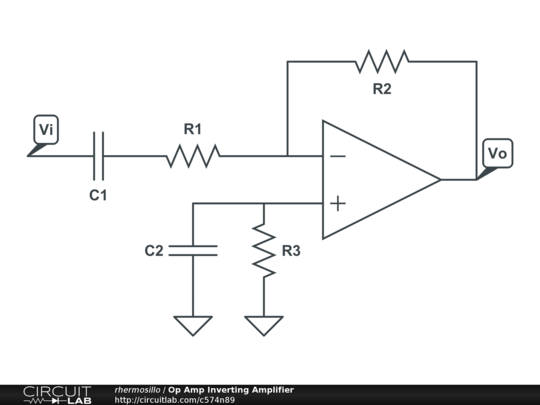
\includegraphics[width=0.70\textwidth]{schematics/invertingopampamplifier.PNG}
\end{center}
The op amp's non-inverting input has ideally no input bias current so no current flows through $R_{3}$ or $C_{2}$ and the non-inverting input is at ground potential. Due to the op amp's high open loop gain, the inverting input is also ideally at ground potential so Kirchhoff's Current Law (KCL) relates $v_{i}$ and $v_{o}$ through the inverting input node. There is ideally no input bias current into the op amp's inverting input so the current through the impedance between the input and the inverting input is equal to the current through $R_{2}$. In the passband the series capacitor $C_{1}$ adds minimal impedance so the current through $R_{1}$ is $v_{i}/R_{1}$. This is also the current through $R_{2}$. The $R_{2}$ terminal connected to the inverting input is at ground potential so the voltage across $R_{2}$ is equal to $v_{o}$. The transfer function is therefore

\textcolor{red}{
\begin{equation}
\frac{v_{o}}{v_{i}} = -\frac{R_{2}}{R_{1}}
\label{eq:invertingopampamplifier}
\end{equation}
}

$R_{3}$ is an optional resistor used to reduce the inverting amplifier's output DC offset error due to a real op amp's nonzero input bias currents. Its purpose is to introduce a small DC offset voltage at the non-inverting input which is equal to the small DC offset voltage at the inverting input. It should be set to

\textcolor{red}{
\begin{equation}
R_{3} = R_{1}||R_{2}
\end{equation}
}

$C_{2}$ is an optional capacitor used with $R_{3}$ to reduce high frequency noise added by $R_{3}$. $R_{3}$ is only needed to produce a DC offset and has no effect on the signal's transfer function, but it produces white thermal noise that can be attenuated by the low pass filter formed by $R_{3}$ and $C_{2}$.
\par The bandwidth of this amplifier depends on the gain since voltage feedback op amps have a constant gain-bandwidth product -- increase the gain and the bandwidth decreases, decrease the gain and the bandwidth increases. If the gain-bandwidth product of the application circuit exceeds the op amp's gain-bandwidth product, multiple op amp inverting (or non-inverting) amplifiers with lower individual gains can be cascaded to achieve a high overall gain but a high bandwidth. The op amp gain is also restricted in most cases to greater than unity since many op amps are unstable for a gain less than unity.
\par One important characteristic of this amplifier is that the gain is determined by a ratio of resistors, which makes the circuit very insensitive to temperature if the resistors are manufactured by the same process. All circuit elements are temperature dependent (resistors included) but since the gain is determined by a ratio of resistors the change in resistance of one resistor due to temperature should be very similar to the change in resistance of the other and the gain undergoes no net change. The op amp itself will exhibit temperature dependencies that affect the operation of the circuit, but modern op amps are designed to have very low temperature drifts so the op amp usually will not cause the circuit to become overly temperature sensitive.

\section{Non-inverting amplifier}
\begin{center}
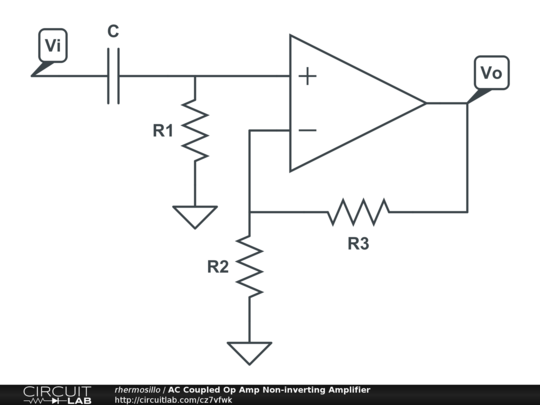
\includegraphics[width=0.70\textwidth]{schematics/noninvertingopampamplifier.PNG}
\end{center}
The op amp non-inverting amplifier also employs negative feedback, but in this case the input voltage is connected to the op amp's non-inverting input. The gain equation is slightly different:

\textcolor{red}{
\begin{equation}
\frac{v_{o}}{v_{i}} = 1+\frac{R_{2}}{R_{1}}
\label{eq:noninvertingopampamplifier}
\end{equation}
}

As with the inverting amplifier, the gain equation can be derived using the fact that an ideal operational amplifier's input terminals are at the same voltage and by using KCL on the inverting input node. Similarly, $R_{3}$ may be replaced with a short but should equal $R_{1}||R_{2}$ to minimize the error caused by the op amp's input bias currents.
\par The gain equation shows that this circuit is a voltage buffer if $R_{1} = R_{2}$, which is as simple as replacing the resistors with wires. The very low output impedance and very high input impedance of op amps ensures the buffer is a good voltage source (which ideally has zero impedance) while not loading down any circuitry that may be generating the desired voltage (such as a voltage divider composed of two resistors).

\section{Inverting summing amplifier}
\begin{center}
	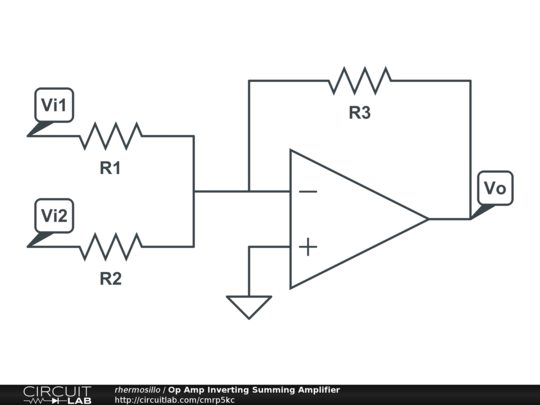
\includegraphics[width=0.70\textwidth]{schematics/invsummingamp.PNG}
\end{center}
\par This circuit multiplies each input voltage by a factor determined by a resistor ratio, sums these amplified voltages, and inverts the result. It is essentially an op amp inverting amplifier with multiple inputs. It is often used as an audio mixer, where multiple voltage signals must be combined into one (for example, voltage signals from microphones near a band's singer and each of its musical instruments must be combined into one signal for recording). The transfer function can be found by superposition of the inputs and, for the two input case, is

\textcolor{red}{
\begin{equation}
v_{o} = -\left(\frac{R_{3}}{R_{1}}v_{i1} + \frac{R_{3}}{R_{2}}v_{i2}\right)
\label{eq:invertingsummingamplifier}
\end{equation}
}

%\par To minimize the error due to the op amp's input bias currents $R_{5}$ should equal $R_{1}||R_{2}||R_{3}||R_{4}$.

\section{Non-inverting summing amplifier}
\begin{center}
	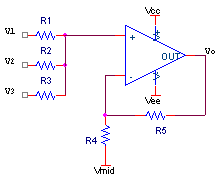
\includegraphics{schematics/summingamp.PNG}
\end{center}
The non-inverting summing amplifier is similar to the op amp non-inverting amplifier, except that it has multiple inputs. To analyze it, note that the inverting input voltage $v_{-}$ is

\begin{equation}
v_{-} = \frac{R_{4}}{R_{4}+R_{5}}v_{o}
\end{equation}

\noindent (assume for simplicity that $v_{MID} = 0$V) since $R_{4}$ and $R_{5}$ form a voltage divider. This is also the voltage at the non-inverting input and KCL can be used on the currents through the input resistors. This gives the transfer function:

\textcolor{red}{
\begin{equation}
v_{o} = \frac{R_{4}+R_{5}}{R_{4}\left(\frac{1}{R_{1}} + \frac{1}{R_{2}} + \frac{1}{R_{3}}\right)}\left(\frac{v_{1}}{R_{1}} + \frac{v_{2}}{R_{2}} + \frac{v_{3}}{R_{3}}\right)
\label{eq:summingamp}
\end{equation}
}

Determining the correct resistor values to use in order to achieve the desired gain for each input (and finding the standard resistor values that will do it) is slightly trickier than the inverting summing amplifier's case. For audio circuits the inverting summing amplifier is easier to work with since a voltage signal that has been inverted cannot be distinguished by the human ear from the same signal that has not -- only amplitude and frequency matter in this case, not phase. Other applications may also allow for an inversion, but if not the non-inverting summing amplifier works well.

\section{Difference Amplifiers}

\subsection{Basic difference amplifier}
\begin{center}
	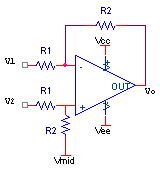
\includegraphics{schematics/differenceamp.PNG}
\end{center}
In this configuration each of the two inputs is connected to one of the op amp's inputs through a resistor ($R_{1}$). Two additional resistors are used: a feedback resistor from the output to the inverting input of the op amp, and another resistor of equal value from the non-inverting input of the op amp to the common mode voltage (usually $V_{CC}/2$ for a single supply system and $GND$ for a dual supply system). Using the fact that an ideal op amp's inputs are at equal voltages and KCL on both the inverting and non-inverting inputs, the transfer function is

\textcolor{red}{
\begin{equation}
v_{o} = \frac{R_{2}}{R_{1}}(v_{2}-v_{1})
\label{eq:differenceamp}
\end{equation}
}

\subsection{High common-mode range difference amplifier}
\begin{center}
	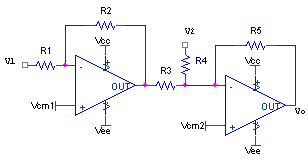
\includegraphics{schematics/highcmdifferenceamplifier.PNG}
\end{center}
This improved difference amplifier allows for a higher common-mode range because the resistors in series with the signal inputs $v_{1}$ and $v_{2}$ ($R_{1}$ and $R_{4}$, respectively) limit the currents into the op amps' inputs, increasing the voltage range within the op amp's drive capability.\footnote{Mancini, Ron., "Op Amps for Everyone", Texas Instruments, Inc., 2002, p. 418} The transfer function can be derived easily using superposition and the above transfer functions for inverting and non-inverting op amp amplifiers to determine $v_{o}$ in terms of all four inputs ($v_{1}$, $v_{2}$, $V_{CM1}$, and $V_{CM2}$). For $v_{1}$,

\begin{equation}
v_{o} = \frac{R_{2}}{R_{1}}\frac{R_{5}}{R_{3}}v_{1}, v_{2} = V_{CM1} = V_{CM2} = 0
\end{equation}

\noindent (the output of the first op amp is $-\frac{R_{2}}{R_{1}}v_{1}$, which is then amplified by $-\frac{R_{5}}{R_{3}}$). For $v_{2}$,

\begin{equation}
v_{o} = -\frac{R_{5}}{R_{4}}v_{2}, v_{1} = V_{CM1} = V_{CM2} = 0
\end{equation}

\noindent For $V_{CM1}$,

\begin{equation}
v_{o} = -(1+\frac{R_{2}}{R_{1}})\frac{R_{5}}{R_{3}}V_{CM1}, v_{1} = v_{2} = V_{CM2} = 0
\end{equation}

\noindent For $V_{CM2}$,

\begin{equation}
v_{o} = (1+\frac{R_{5}}{R_{3}||R_{4}})V_{CM2} = (1+\frac{(R_{3}+R_{4})R_{5}}{R_{3}R_{4}})V_{CM2}, v_{1} = v_{2} = V_{CM2} = 0
\end{equation}

\noindent Putting it all together,

\textcolor{red}{
\begin{equation}
v_{o} = \frac{R_{2}}{R_{1}}\frac{R_{5}}{R_{3}}v_{1} - \frac{R_{5}}{R_{4}}v_{2} - (1+\frac{R_{2}}{R_{1}})\frac{R_{5}}{R_{3}}V_{CM1} + (1+\frac{(R_{3}+R_{4})R_{5}}{R_{3}R_{4}})V_{CM2}
\label{eq:highcmdifferenceamplifier}
\end{equation}
}

\noindent If all the resistors are equal, the transfer function simplifies to

\textcolor{red}{
\begin{equation}
v_{o} = v_{1}-v_{2}-2V_{CM1}+3V_{CM2}
\label{eq:highcmdifferenceamplifier_simple}
\end{equation}
}

\section{Differentiator}
\begin{center}
	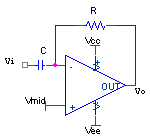
\includegraphics{schematics/differentiator.PNG}
\end{center}
The differentiator is similar to the inverting op amp amplifier except that there is no resistor in series between the input and the op amp's inverting input -- only a capacitor is used. The inverting input's voltage is equal to $v_{MID}$, and KCL on this node can be used along with a capacitor's I/V relationship ($i_{C} = C\frac{dv_{C}}{dt}$). The transfer function is thus

\textcolor{red}{
\begin{equation}
v_{o}(t) = -RC\frac{dv_{i}(t)}{dt}
\label{differentiator}
\end{equation}
}

\noindent Another way to represent the transfer function is with complex numbers:

\textcolor{red}{
\begin{equation}
\frac{v_{o}}{v_{i}}(s) = -sRC = -\jmath \omega RC
\label{eq:differentiator_complex}
\end{equation}
}

Unfortunately, the differentiator suffers from a high frequency noise problem; the circuit naturally amplifies high frequency signals so the output will oscillate unless all high frequency signals at the input are sufficiently attenuated. Since noise typically has high frequency components it can be very difficult to stabilize this circuit.
\par One way to avoid the unwanted amplification of high frequency signals or noise is to place a resistor in series with the capacitor. This, of course, gives the differentiator the same topology as the op amp inverting amplifier! The difference is that the op amp inverting amplifier uses a much larger AC coupling capacitor to block very low frequency signals whose frequencies are below the range of frequencies the circuit is meant to operate on, while the capacitor in the differentiator is smaller to affect the appropriate range of frequencies. Reusing the analysis of the op amp inverting amplifier but replacing the input resistor with the impedance of the input resistor and capacitor, the transfer function (using the complex s) is $v_{o}(1+R_{I}C) = -sRCv_{i}$. If $R_{I}C$ is much less than the period $T$ of the signals the circuit must operate on, however, the equation simplifies to

\textcolor{red}{
\begin{equation}
\frac{v_{o}}{v_{i}}(s) \approx -sRC
\label{eq:differentiator_series_cap}
\end{equation}
}

which is the same as before.\footnote{Johnson, David E., "Operational Amplifier Circuits: Design and Application", Prentice-Hall, 1982, pp. 79-80}

\section{Integrator}
\begin{center}
	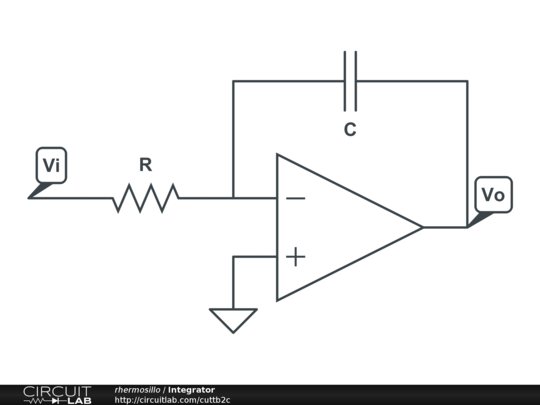
\includegraphics[width=0.70\textwidth]{schematics/integrator.PNG}
\end{center}
The integrator is very similar to the differentiator -- just switch the resistor and capacitor. Using impedance and KCL again, the transfer function is

\textcolor{red}{
\begin{equation}
v_{o} = \frac{-1}{RC}\int v_{i}dt\ = \frac{-v_{i}}{sRC} = \frac{-v_{i}}{\jmath \omega RC}
\label{eq:integrator}
\end{equation}
}

The integrator does not suffer from the same high frequency noise issues as the differentiator since it naturally attenuates high frequency signals.

% TODO
%\section{Op Amp Current Doubler}
% see p. 17 of the OPA454 datasheet. Slave amplifier is essentially a buffer in parallel with an op amp circuit (in any configuration)
% also add somewhere that you can add a class B push-pull output stage to increase the current output of the op amp (see also p. 17 of the OPA454 datasheet)
